\documentclass[10pt,twocolumn,letterpaper]{article}

% Prevent words from being hyphenated
\hyphenation{OpenOffice}

\usepackage{fullpage}
\usepackage{graphicx}

\author{David Simon}
\title{Task-Specific Filesystem Block Reorganization in Ext3}

\begin{document}

\maketitle

\begin{abstract}
Hard disk access times are the most significant performance bottleneck when
starting typical applications on contemporary personal computers and servers.
Most modern programs must load numerous libraries, resource files, modules, and
other pieces of information off disk before performing any useful work. Optimization
in this area should prove fruitful.

We attempted to reduce the amount of time consumed by hard disk activity during
the initialization of various programs. To do this, we observed which data blocks were
used during the initialization of various programs. Then, those blocks were moved
closer together, in the hope that the quantity and length of drive head seeks
would be reduced. The results were mixed; some applications received no particular
benefit from this optimization, while others started significantly faster.
\end{abstract}

\section{Introduction}

Hard disk drives are, by a wide margin, the slowest internal storage devices commonly
used in modern computing. For a typical read or write, the disk head must first
\emph{seek} to the target block\cite{seektime}. On even the fastest hard disks\cite{deskstar}, one seek
can take several milliseconds, often orders of magnitude longer than the operation which will actually
use that data. Even if seeking is unnecessary because the disk head is already at the correct track, there is
often still a long delay waiting for the desired block to spin around to the head again\cite{latency}. When
many disk operations are required, tasks that would otherwise be immediately performing computations on data must first wait for these slow, mechanical processes to complete.

Ideally, to mitigate this problem, the next block to be requested should be physically near to
and after the current block\cite{autolocality}. When seeking or spin latency is unavoidable, then it is better if the travel time required can at least be lessened by reducing the
physical distance between the current block and the next. The best scenario is when
as much disk time as possible is spent actually retrieving data, and as little as possible
wasted travelling from one request location to another.

It should be possible, with intelligent organization of data on the disk, to make the hard drive behave
more closely to this ideal. Bolero, the Block Organizer that Localizes Empirically-Related Objects, was developed as a proof-of-concept for this idea.

\section{Motivation for Bolero}\label{sec:motive}

In most filesystems, files are divided up
into one or more fixed-size chunks, called \texttt{blocks}CITETHIS. When a file's blocks
are not contiguous on disk, then the file is \texttt{fragmented}
and operations that require more than one block from the file are slow due to
seek and spin delays. The best proactive way to prevent fragmentation is to find contiguous
chunks of available space when allocating new files. Some older filesystems, such as FAT, were
very ineffective at doing this\cite{fathistory}.
FAT filesystems frequently had to be \texttt{defragmented} to maintain performance.
Modern filesystems, such as NTFS CITETHIS and ext3 CITETHIS, keep better track of free space,
and do not tend to fragment until the filesystem becomes nearly full. Advanced filesystems sometimes
use even more sophisticated strategies to prevent fragmentation, such as preallocating extra room to allow 
contiguous appending, or delaying physical allocation as long as possible so that better guesses
can be made about the characteristics of newly created files\cite{xfs}.

As important as these advancements have been, however, they do not address another, more subtle form of fragmentation: fragmentation between related files.
Just as slowdowns result when the various blocks of a file are distant from each other, when \emph{files} accessed in sequence are far from each other on the disk, significant unnecessary delays may result. For example, a large application such as an office suite or desktop environment requires numerous programs, shared libraries, icons, fonts, and other resources before it can start up completely. If these files must be read from disk but are spread apart from each other, the application's startup time will increase.

The objective of Bolero is to reduce this type of fragmentation for that specific case, that of applications
starting up and loading a variety of resources from disk. It accomplishes this by moving data blocks that are accessed at about the same time closer together, and re-sequencing them into the order they are expected to be accessed. There are two possible strategies to accomplish this: general optimization and task-specific optimization.

With general optimization, the reorganizer would use the recorded observations
to determine which files tend to be accessed within a short time from each
other, and in what order. It would then place files on disk in such a way as
to reduce average seek time and spin latency throughout the computer's operation.
Previous attempts at implementing this type of optimization at a
sub-filesystem level have resulted in significant performance benefits\cite{autolocality}.

The other approach, task-specific optimization, is simpler to
implement and may also (for its specific purpose) result in better performance. With this
approach, observations are limited to a particular, short-term task. For example,
the objective may simply be to get the computer's desktop environment to load
quicker after a cold boot. Within a short but disk-intensive period like this, even
though there will have been a lot of disk activity, any single file will
probably have been read from disk only once. The reorganizer can therefore simply
rearrange the relevant files on the disk to be contiguous and in the same order as that
recorded during the observational period, to reduce the amount of time taken for
that particular task. Previous efforts using this approach have been
successful in reducing large application startup times by over 60\%\cite{ala}.

Because task-specific optimization is easier to implement and readily suggests
a metric, we chose it as the approach used by Bolero. However, since that approach is a
specialization of the general optimization approach, its success may be seen
as a motivation to explore the more complex, but potentially more rewarding, area
of general optimization.

For this project, we attempted to improve the startup time of the following applications with this approach:
\begin{itemize}
\item X Windows + KDE
\item OpenOffice
\item MySQL
\end{itemize}
Among these three applications, a wide range of shared libraries, subsystems, and user interface types
are involved. This helps to eliminate the influence of these factors on the final results;
ideally, the only factor being tested should be disk usage.

The test environment was a default installation of Kubuntu 8.04 on a 12GB partition located
at the end of the 61.4GB test hard disk, a PATA Maxtor 6Y060L0. The test system had
1GB of RAM, and a 2.4Ghz processor. This combination of a somewhat powerful system and
a somewhat mediocre hard drive was chosen purposefully: this scenario exacerbates the
problem of the hard drive as the bottleneck of the application loading process, and therefore
any improvement due to the optimization process should be especially noticeable.

\section{Filesystem Manipulation}

Because of the relative ease of extending and manipulating Linux filesystems and
kernel code, Bolero was be developed targetting Linux environments with ext3
filesystems. Ext3 is the standard filesystem used in Linux
environments, and is largely backwards compatible with ext2\cite{ext2journal}.
The general approach used by Bolero, however, is also applicable to most other commonly-used
filesystems.

The basic mechanism used by Bolero is the \texttt{libext2fs} library. This C
library, part of the standard \texttt{e2fstools} package, allows user-space programs
to open, scan, and make changes to ext2 filesystems. To make development simpler, we wrote
a Python wrapper called \texttt{pyext2} around a subset of this library's functionality.
This library can open and scan through an ext2 or ext3 filesystem, report
various information about its contents, and swap the locations of arbitrary data
blocks while maintaining the filesystem's internal consistency. With this library,
it was easy for us to write a wide variety of quick Python scripts to accomplish
a variety of filesystem-related tasks.

Although there are some tentative mechanisms to allow the online rearrangement
of ext3 blocks\cite{ext3online}, Bolero is designed to run only on unmounted filesystems.
While it would be
convenient for the user to be able to manipulate a mounted filesystem, doing so
would add unnecessary complexity, making debugging and
development more difficult than necessary. Working with unmounted filesystems,
the reorganizer code can stay entirely in user-space, and does not have
to deal with the possibility of the file system's state being changed
midway through the process by other mechanisms outside its control.

With only the basic tool of swapping data blocks, a wide range of possible
defragmentation techniques are possible. Bolero includes \texttt{defragment.py}
a very simplistic, traditional defragmenter for ext3, which
does nothing but reduce fragmentation within individual files. Because ext3 files do
not usually tend to fragment, the case for this kind of reorganization alone
is not very strong. However, individual file defragmentation is an important
basis for later, more sophisticated operations, and also serves as a useful test
of the system's ability to safely and correctly alter filesystems.

Once the reorganizer can reduce file discontiguity, it is possible to
use that same mechanism to reduce inter-file discontiguity, as explained
in section \ref{sec:motive}. Both types of defragmentation are necessary because the overall goal is to reduce the quantity of seeks and increase contiguity. The ideal state of affairs is for the disk to travel through
a sequence of files without interruption\cite{autolocality}, from the first block of the first file to the last
block of the last file with no delays or seeks.

This ideal is difficult to achieve completely, due to the realities of hard disk
and filesystem layout. For example, in ext3, data blocks are organized into larger
collections on disk called \texttt{block groups}\cite{ext2intro}. Each
block group contains actual data blocks as well as other information, such
as bitmaps describing available space, and tables of \texttt{inodes},
which describe meta-data for each file. These areas of meta-information within
groups create ``gaps'' of disk area which the defragmenter cannot
use to reduce discontiguity, because there can never be file data there.
The current implementation of Bolero ignores this problem and simply
skips over these gaps. A more subtle defragmenter might attempt to arrange
files around these gaps in anticipation of access patterns.

There are many other issues which present similar complications to a defragmentation
system, such as track boundaries, unusual varieties of file data (i.e. directories, which
are almost never scanned through linearly), and files which are expected to change
size or be deleted during normal operations. The Bolero defragmenter makes no attempt to
solve even these relatively common complications.

However, even an unsubtle implementation such as Bolero can serve as a proof-of-concept
to demonstrate the validity of the basic idea. If a repeatable, significant improvement
is observed after making simplistic improvements to the filesystem layout, it follows
that more sophisticated improvements should yield even better results.

\section{Observing Disk Activity}\label{sec:observing}

The major difference between the Bolero defragmenter and a traditional defragmenter
is that information about the relationships between files (specifically, the order
in which tend to be are accessed during specific tasks) is used. We developed a few
simple observation tools to record such information. These same tools were also used to record
timing information for each of the target tasks, in order to determine how much improvement
the optimization process was yielding, as described in section \ref{sec:results}.

For each task in each state (either the untouched control state or an optimized state), the
following procedure was used to collect observational data:
\begin{enumerate}
\item A \texttt{proc}-based mechanism is used to clear the Linux system's software-based disk cache. CITETHIS
\item Thirty MB is read from the beginning of the target drive, far from the target filesystem, in order to deceive the drive's internal cache. Without this step, test results tended to change as subsequent tests were performed, as the drive restored information from its cache rather than seeking to and reading the physical data itself.
\item If applicable, a tool called \texttt{frecord} is started, which would monitor for new processes starting up and record which
files they opened.
\item A timestamp is taken, and the target program is started.
\item When the program is finished loading (the definition of which is dependent upon the particular program being observed), the elapsed time is recorded, and \texttt{frecord} is stopped if it had been started earlier. It is at this
point that \texttt{frecord} writes its collected information to disk.
\item The target program is terminated, and the procedure can begin again.
\end{enumerate}

For each target program, this procedure was repeated 100 times. For each run of the procedure, the \texttt{frecord}
process noted which processes started up after its initialization. Every 3 milliseconds, the open files of each
of these processes were recorded to memory. Afterwords, the information in these 100 recordings of file usage
was collected by the \texttt{fsummarize} tool, which uses it to produce a best-guess list of all the files
that might be opened the next time the target application starts up, in the order they are most likely to be
opened in. All files which were opened in even one of the recorded sessions are included in the list. In theory,
it is better to include an unnecessary file and have the disk head skip over it with relatively little expense than to omit it and force the disk to (even occasionally) perform an expensive seek to some other part of the disk
and then back.

\section{Defragmentation}

There are two defragmenters included with Bolero that can make use of the results from \texttt{fsummarize}:
\texttt{defragment.py} and \texttt{mdefragment.py}. The former locates every data block for every file mentioned
in the summary, and puts them in sequential order on disk, starting at the first block of the group containing
the first inode. The latter, \texttt{mdefragment.py}, acts in a similar way, but instead starts at the group containing the mean from all inodes involved. This was done as an attempt to reduce the average seek distance for
those remaining seeks which must be performed, particularly seeks to inode table entries (see section \ref{sec:future}).

After defragmentation, the blocks that were originally in the area that the task-related blocks were sorted to
are strewn arbitrarily around the disk. This is acceptable for the purposes of this project, since those (now
discontiguous) files are unlikely to be accessed during the target task at all; if the target application being observed loads the same functionality every time it is started, and a file hasn't been noticed
in even one of the 100 \texttt{frecord} observational runs on that application, then it's a safe assumption that that file is not related to the application's loading process. However, the file may still be need for some other application or task. For that reason, a Bolero-like approach applied to a production system would have to be more considerate of those data blocks it must move out of the way.

\section{Measuring Results}\label{sec:results}

In order to gauge how successful any optimization is, it is important to have
repeatable, objective measurements. For the specific task that Bolero was written
to address, optimizing the startup time of various applications, this means that it
is necessary to have a way to accurately measure the amount of time it takes for
a program to startup, and then to perform that measurement a significant
number of times on both a control filesystem and a filesystem optimized for that program.

% This figure is up here in this weird spot so that it appears at the top of the page describing the
% related results. LaTeX can sometimes be too smart for its own good.
\begin{figure*}[!htb]
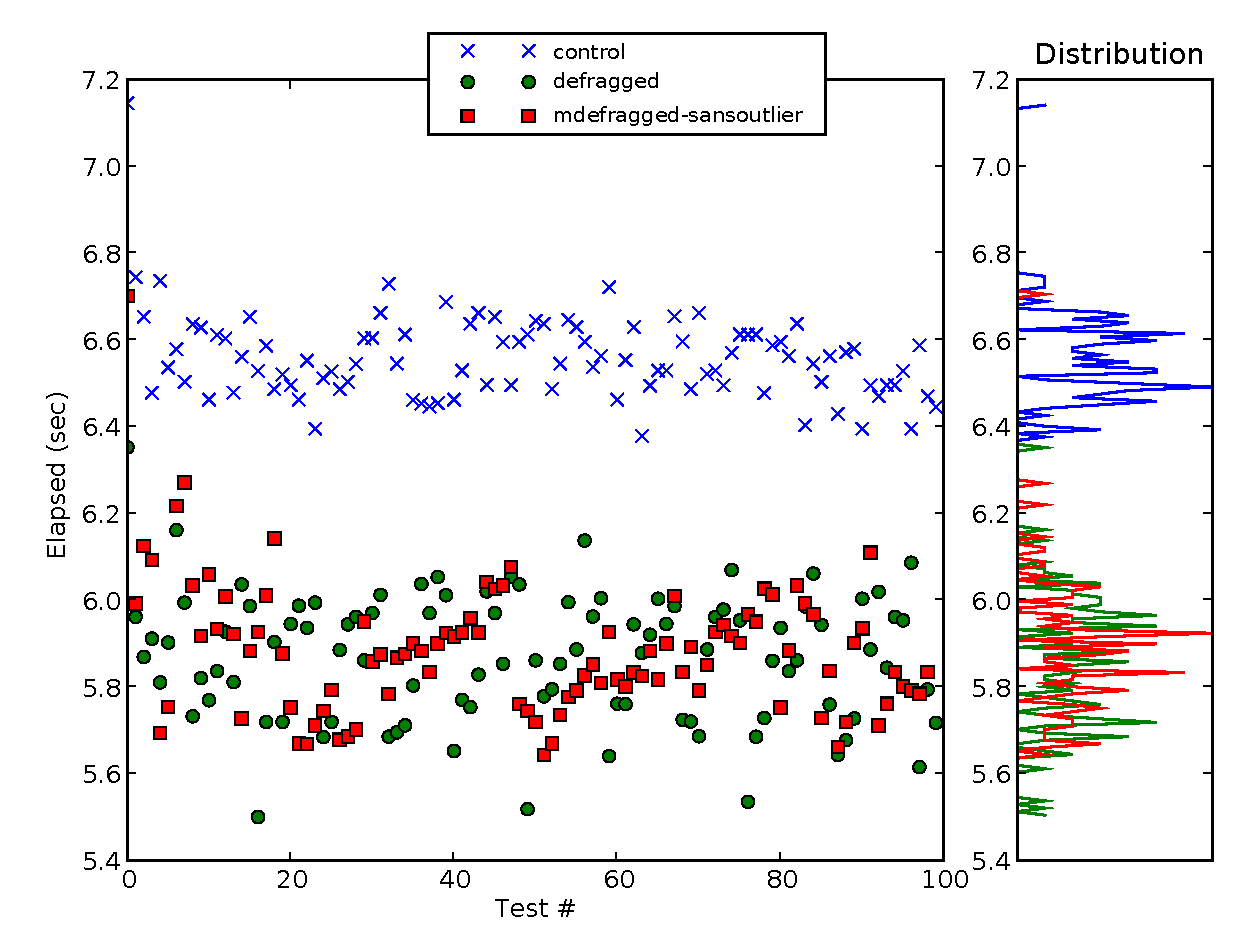
\includegraphics[scale=0.75]{mysql-chart.eps}
\caption{Startup times for MySQL}
\label{mysqlchart}
\end{figure*}

However, this measurement is more ambiguous than we initially expected, and a few
somewhat arbitrary choices had to be made. The most important of these is the problem of determing when, exactly,
a program has ``started up'' entirely. For some programs, this is fairly straightforward to define. For example,
MySQL has started up entirely when it is able to successfully respond to SQL requests. Therefore,
to determine the startup point for MySQL, the measurement program merely has to act
as a MySQL client, perform a query, and mark the time at which MySQL is able to
respond with the correct results.

For GUI programs, however, the startup point is more nebulously defined ``as when the user is
able to interact with the program''. OpenOffice, for example, is considered by Bolero to have started up completely when it has opened up and ran a macro within a document supplied to it as a command line argument. This is an arbitrary decision, but as long as it includes a good amount of the application's disk-related initialization activity, and as long as the same standards are applied to both the control and the optimized filesystems,
it suffices.

For each target program, once this issue of finding a measurable ``ready'' point was solved,
the same experimental procedure could be applied to each:

\begin{enumerate}
\item The target filesystem being tested is restored from backup to an unoptimized control state.
\item A control measurement of 100 samples is taken as described in section \ref{sec:observing}, with \texttt{frecord} disabled. This data is the baseline for how long the application takes to start up
on the filesystem before optimization.
\item This measurement is then repeated 100 more times, but with \texttt{frecord} enabled.
\item The results from \texttt{frecord} are supplied to \texttt{defragment.py}, and the filesystem is now optimized with task-related data blocks contiguous and sequential near the first related inode.
\item Another 100 timing samples are taken with \texttt{frecord} disabled.
\item The target filesystem is restored to control state from backup again.
\item The filesystem is optimized again, using the same \texttt{frecord} results, but using \texttt{mdefragment.py} instead.
\item Another 100 timing samples are taken, again with \texttt{frecord} disabled.
\end{enumerate}

This provides a clear picture of how well the two defragmentation strategies affect the application's startup time. The results for each application are described in more detail in the following sections.

% This figure is up here in this weird spot so that it appears at the top of the page describing the
% related results. LaTeX can sometimes be too smart for its own good.
\begin{figure*}[!htb]
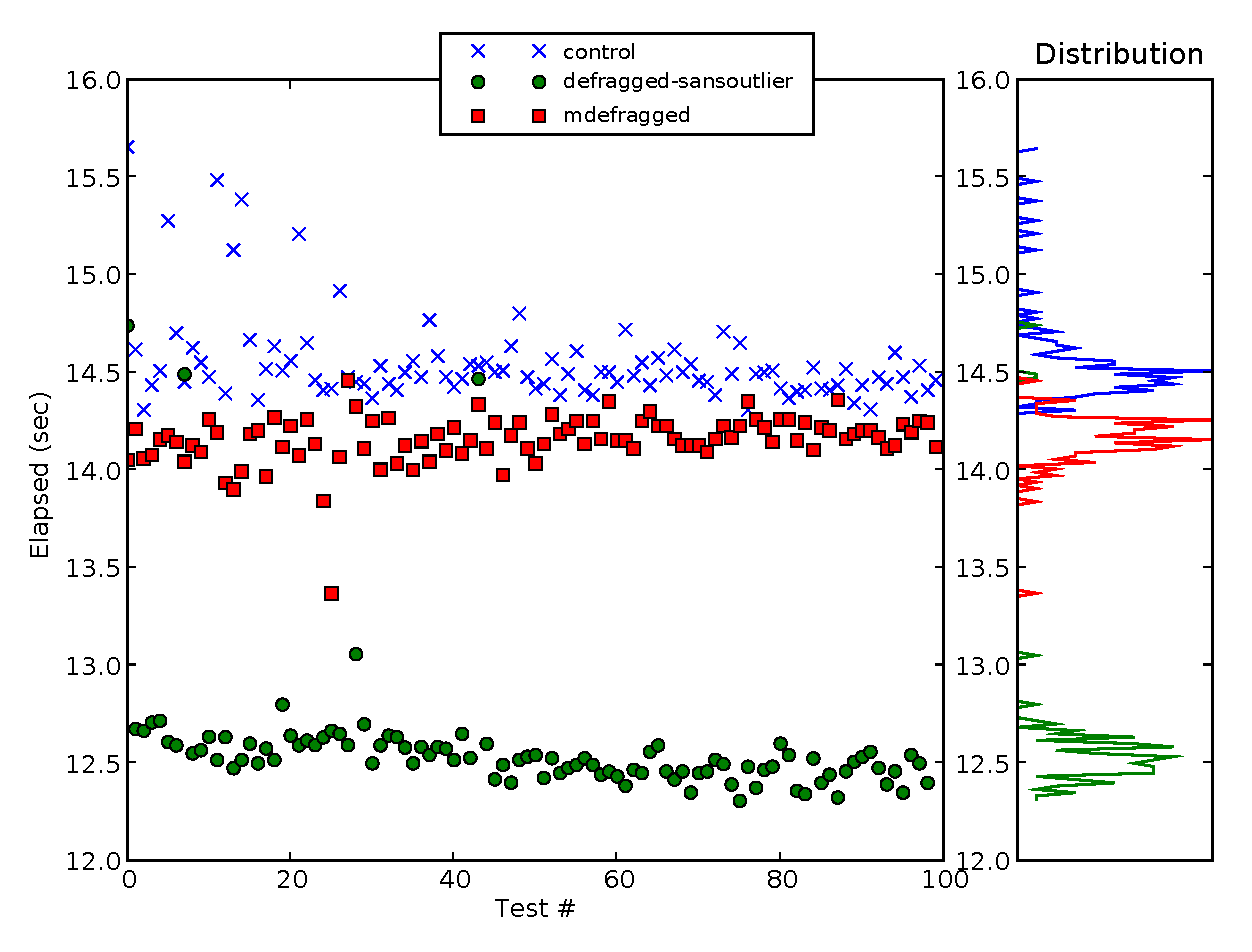
\includegraphics[scale=0.75]{openoffice-chart.eps}
\caption{Startup times for OpenOffice}
\label{oochart}
\end{figure*}

\section{Data Collected for MySQL}

As noted in section \ref{sec:results}, server applications such as MySQL are easy to measure because it is easy to define the point at which they have ``started up'': when they are able to serve client requests.

For measurement purposes, a sample database containing two related MyISAM tables with various column types and indexes was defined. These tables were filled with 20,000 and 10,000 lines of pseudo-random data respectively. Although this data was randomly generated, it was only generated once; that is, although the data was arbitrary, both the control and experimental tests were operating on the \emph{same} arbitrary data.

The timing process, for each sample, takes a beginning timestamp, calls the init.d script for MySQL, and waits for it to return control. Then, it connects to the server using the Python \texttt{MySQLdb} client module, and supplies it with a complex query involving data and indexes for both tables. The query is limited to return 10 rows, and once the
server supplies those rows to the client, the ending timestamp is taken. The results of these timings are shown in Figure \ref{mysqlchart}.

The mean time elapsed between beginning and ending timestamps for the control was 6558.43 ms, with a standard deviation of 99.82 ms. The \texttt{frecord} observations for MySQL yielded a sequence of 142 files, including the database files themselves, the various programs and libraries used by MySQL, and those resources used by the init.d script. After those files were defragmented with \texttt{defragment.py}, the mean time elapsed decreased by nearly a second to 5873.32 ms, with a standard deviation of 147.24 ms. The results after defragmentation with \texttt{mdefragment.py} were very similar, with a mean of 5884.01 ms and a standard deviation of 152.76 ms, after the removal of one outlier (8237 ms) from the result set.

Thus, both types of defragmentation resulted in a significant change in the mean startup time of MySQL, a reduction of about a full second. The optimization, however, also increased the variance between samples significantly.

% This figure is up here in this weird spot so that it appears at the top of the page describing the
% related results. LaTeX can sometimes be too smart for its own good.
\begin{figure*}[!htb]
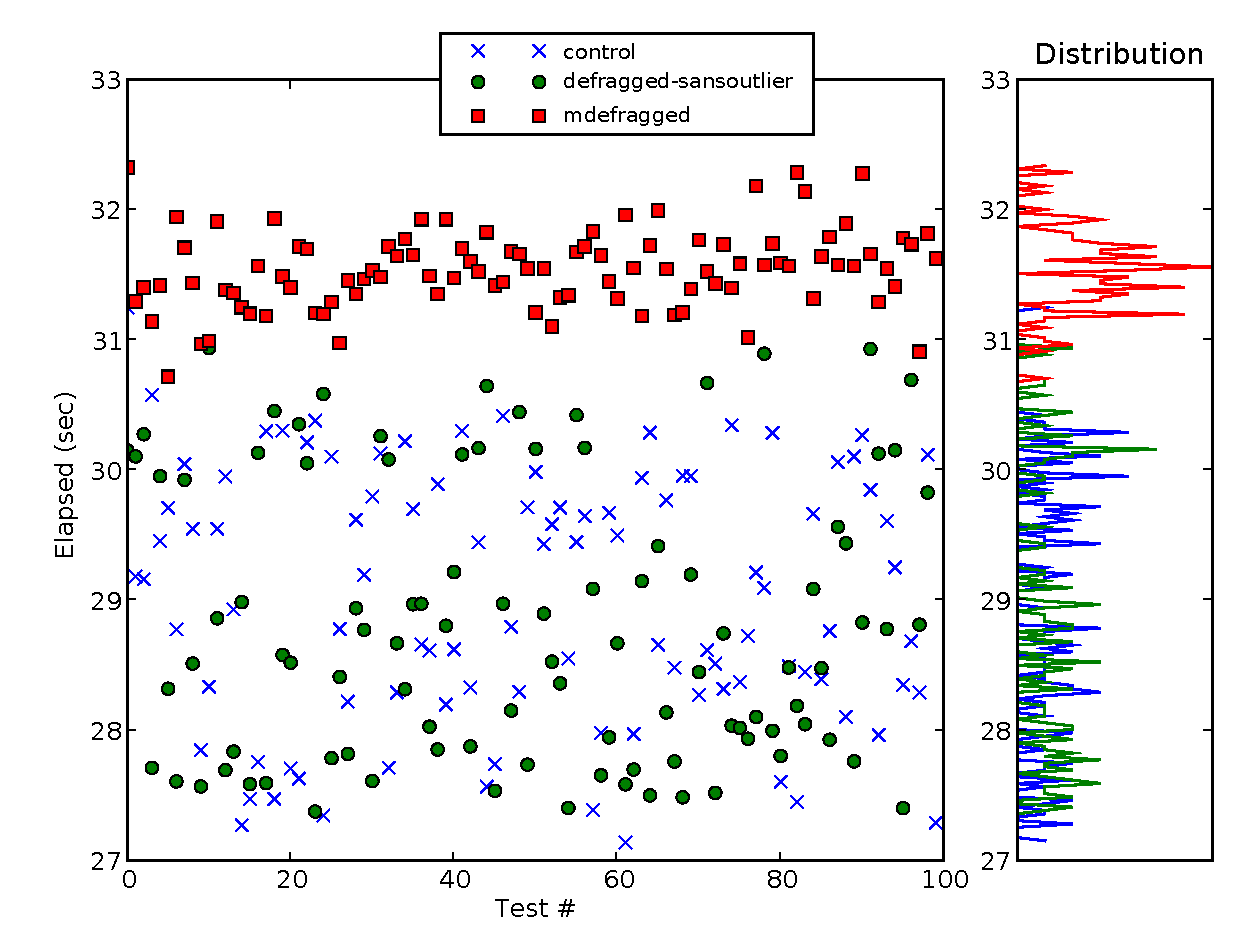
\includegraphics[scale=0.75]{kde4-chart.eps}
\caption{Startup times for X and KDE4}
\label{kde4chart}
\end{figure*}

\section{Data Collected for OpenOffice}

As explained in section \ref{sec:results}, using an automated process to measure the startup time of a graphical application is more complicated than it is for a server. The difficulty is in finding a particular task to give to the program that can be easily tested by the script, that requires a substantial portion of the program to be loaded, and that represents a reasonable point at which the user can stop waiting and begin actually working with the program.

For OpenOffice, we defined the ready point to be the time at which an existing document is opened in the word processor and the user may begin editing it. For this purpose, we created an OpenOffice Writer document which contains a macro. This macro attempts to connect to a socket on the local machine as soon as the document is opened. For each timing sample, the timing process opens this socket, marks a beginning timestamp, and then runs OpenOffice on the test document. As soon as the test document is loaded and makes an attempt to connect to the socket, the ending timestamp is marked. The results are shown in Figure \ref{oochart}. Throughout the process, a X/KDE environment was kept running; only OpenOffice itself was started and stopped.

The mean elapsed time on the control filesystem was 14551.48 ms, with a standard deviation of 232.81 ms. Observations on the control system gave a list of 496 files used by OpenOffice. After
defragmentation of those files with \texttt{defragment.py}, and the removal of a high outlier (31889 ms) from the result set, this mean decreased by about two seconds to 12587.40 ms, and the standard deviation increased to 367.09 ms. After defragmentation by \texttt{mdefragment.py}, the mean only decreased from the control by about 0.4 seconds to 14157.44 ms, with a standard deviation among samples of 128.04 ms.

For OpenOffice, in this particular situation, both defragmenters created an observable improvement in OpenOffice's startup time, but the effect of optimization by \texttt{defragment.py} was much greater than that by \texttt{mdefragment.py}. The standard deviation was also noticeably affected by the optimization process.

\section{Data Collected for X \& KDE}\label{sec:kderesults}

Desktop environments such as KDE are complex systems which run several independent but related processes simultaneously. Such systems have not really started up \emph{entirely} until they are capable of performing every one of their varied functions. It would not be enough to say that KDE has fully loaded when it is, say, possible to use its main menu to launch applications, because at that time KDE might still be busy loading other components, such as the background image manager, or the taskbar, or the file management layer. It would be impractical to test a task for each of these distinct features individually, as we did for the specific goal of ``loading a document'' within OpenOffice, so another method for finding the startup point was needed.

We decided to use the Konqueror web-browser for the timing metric, by having KDE4 start it automatically upon logging in, and directing it to a local port being managed by the test framework. The ending timestamp is taken as soon as the port is opened. This approach was chosen for several reasons:
\begin{itemize}
\item Konqueror depends upon several other KDE components, including its interprocess communication system, and its IO handler system CITETHIS. Therefore, before Konqueror could effectively attempt to contact the test server, a good portion of KDE would have to be loaded first.
\item KDE's auto-start mechanism, which is used to start up user-specified programs automatically each time a new session is started, is activated near the end of the KDE initialization process CITETHIS. By this point, nearly all of X and KDE will have been loaded, or at least started loading.
\item Browsing a webpage is a reasonable choice for a task a user would want to do as soon as possible after starting an X/KDE session. 
\end{itemize}

A user who is starting an X/KDE session in order to open up Konqueror and browse a webpage is working under the same restrictions as the automated timing process. This means that any improvement reported by this metric due to the optimization is an improvement to the actual user-perceived responsiveness of the system. However, this improvement
did not materialize, as can be seen in Figure \ref{kde4chart}.

On the control filesystem, the mean elapsed time was 29022.81 ms, with a standard deviation of 972.04 ms. The file sequence collected from \texttt{frecord} referenced 1201 files. After the \texttt{defragment.py} optimization process, this mean (after the removal of a single outlier from the result set, 46058 ms) decreased only slightly, to 29000.14 ms, and the standard deviation more than doubled to 2011.59 ms. The results from the \texttt{mdefragment.py} process were even less helpful: the mean elapsed time \emph{increased} to 31543.05 ms, with a standard deviation of 300.57 ms.

\section{Analysis of Results}

Among the three applications tested, both MySQL and OpenOffice saw measurable improvements in their startup times, by approximately 14\% and 11\% respectively. X/KDE4, however, received no improvement in its startup time due to the optimization process. Why didn't X/KDE4 benefit as the other applications did? We hypothesize that the difference in effectiveness of the optimizer is due to a major architectural difference between X/KDE and the other two tested applications: the number of simultaneous processes.

MySQL and OpenOffice start up relatively few processes, but an X/KDE4 session involves the creation of many processes, all of which are started in the same short time period. These processes, all running concurrently and attempting to load resources, create a situation that is very different from the ideal disk usage scenario, a single pass read of all necessary resources. Many concurrent requests for different resources on the disk would require that the disk head seek back and forth to fulfill them. This occurs because, even if the optimizer is correctly ordering all data blocks on disk into the order in which the process of reading those blocks \emph{begins}, the disk must still often break away from the predicted sequences in order to continue concurrent, in-progress reads. However, although we feel that this is the most plausible explanation for why optimization of X/KDE4 was ineffective, this explanation should be verified through experiment.

Another odd aspect of the results that we were not expecting was the dramatic change in standard deviation among test results after optimization was applied. In MySQL, the standard deviation increased by about 50\% after both forms of optimization. For OpenOffice, the standard deviation approximately doubled after \texttt{defragment.py} was used, but approximately halved after application of \texttt{mdefragment.py}, and similar effects on the standard deviation were seen when these tools were applied to X/KDE. In particular, we found it surprising that, throughout the results collected, the most effective optimization tended to \emph{increase} deviation, rather than decreasing it. There does not seem to be an obvious explanation for these odd results. It would be difficult to tell if these changing delays are even disk-related without first collecting more detailed information about the disk's behavior during the tests.

One final result that surprised us was that, in all cases, the \texttt{mdefragment.py} tool was \emph{less} effective than \texttt{defragment.py}. This appears to contradict our original theory about why this type of optimization should be effective. Reducing the average seek distance between inodes and their data blocks should have, under that theory, reduced the overall time elapsed. The next step in understanding this issue would be to obtain more detailed information about the disk's internal activity during the tests.

\section{Future Work}\label{sec:future}

We assert that the project, as it currently stands, is enough to demonstrate the basic validity of this approach to disk optimization. However, the project is far from a state where it would be effective in a production setting. As it currently stands, the gains in performance created by the Bolero optimizer are insufficient to outweigh the trouble of applying it. There are many areas in the project where future work could address this problem from both angles: increasing the performance gain, and reducing the administrative hassle of using the system.

Correcting the latter problem, allowing administrators to take advantage of disk contiguity optimization easily, would require addressing two significant problems:
\begin{itemize}
\item Before applications can be optimized, time-consuming file usage recordings must first be taken. During these recordings, the application is being repeatedly started and stopped, and other applications should not be running. During this long period, therefore, the system is useless for actual production work, and that is unacceptable in many scenarios.
\item The filesystem cannot be optimized while it is mounted. Therefore, if a system-critical partition is to be optimized (and, since Bolero is meant to optimize major applications, this is likely), the system must be brought down and booted from an alternate partition. The defragmentation process itself is also fairly slow, and no production work can be done with the target filesystem while it is being defragmented.
\end{itemize}

These problems are particularly troublesome considering that filesystems often change, necessitating that the entire sequence be re-done if benefits are to be maintained. The current implementation of Bolero assumes that it can place a data block down in a particular spot on disk and rely on it staying there, but there are many reasons why this assumption is invalid. The most obvious of these is that production filesystems tend to change as time passes. Log files expand and are rotated, databases are manipulated, libraries and programs undergo regular updates, and so on. In a typical filesystem, no file can be relied upon to stay in one place or one state forever, but this is exactly the assumption that the Bolero optimizer makes.

An improved optimization system could correct this problem somewhat by re-optimizing the filesystem continuously or at regular intervals, but the ideal solution would also involve giving the optimizer more information about the \emph{purpose} of files. This information could allow an improved version of Bolero to predict which files are likely to be deleted or expanded or changed in other ways, and which files will most likely stay unaltered for long periods of time. With this information, the optimizer could allocate extra space as needed to allow such changes to occur without affecting on-disk contiguity.

However, this still doesn't address the chief problem with Bolero in its current state: the long time periods during which the filesystem is being measured or defragmented, and therefore cannot be used productively. We propose that the solution to this issue is two-fold: the file usage data must be gathered on development systems rather than the production system, and it must be possible to optimize a running filesystem without interrupting its work. After these improvements, the process of optimizing (or re-optimizing) a particular application might be as follows:
\begin{enumerate}
\item A new application, or a new version of some existing application, is released. The administrator of a production system wishes to install it on disk in an optimized fashion, so that its start-up time is as short as possible.
\item The administrator fetches and installs the new application, and additionally obtains information describing its expected file usage patterns. This information was prepared by the administrator on a non-critical development system. Or, alternately, perhaps this information was prepared in advance by the application's developers, and included with the new release.
\item The administrator gives the optimizer this file usage information, and the optimizer defragments the filesystem in-place, without unmounting it or interrupting it.
\end{enumerate}

The first major change presented in this scenario is the source of the file access information; instead of being generated by the administrator on the target machine, it's created on some other machine and possibly by an entirely different person. This requires little or no change to the technology itself; although a given application may be installed differently on each machine, the process of starting it up should be about the same on all machines. Depending on the application, there may be optional components that are loaded or not loaded on a per-system basis, but this is easy to work around: as long as the file access information is as comprehensive as possible, particular files which are listed in that information but not found on the target filesystem can simply be skipped over, and contiguity is maintained.

The second change in the above scenario, however, is more involved: the optimizer must be able to act on live filesystems. This would require abandoning the current \texttt{libext2fs}-based mechanism, which requires that the filesystem be unmounted while it is altered. However, existing mechanisms exist in the Linux kernel for manipulating filesystems at a deep live while they are mounted\cite{ext3online}, and Bolero could most likely be adapted to use those.

The improvements listed above, if implemented, would do much to deal with the administrative barrier-to-entry of the system. However, there is also a great deal of room for possible further work on the other side of the system: the effectiveness of the optimization itself.

A significant property of both Bolero reorganizers is that \emph{only data blocks} are moved; inodes are
unaltered by the process. This is because the \texttt{pyext2} library included with Bolero is incapable of moving inodes.  A given file's inode entry must be read first to locate its data blocks. Therefore, depending upon how scattered the inodes are on disk and in what order are read, their placement is almost certainly a significant remaining source of optimizable disk delays and seeks. This is the most significant theoretical problem remaining with the project, and we suspect that implementation of inode defragmentation would increase the effectiveness of the optimization a great deal.

In particular, we suspect that implementing inode defragmentation would help the optimization to be more effective in scenarios such as the X/KDE test described in section \ref{sec:kderesults}. Bolero was able to move data blocks related to X and KDE files from 34 block groups scattered around the test filesystem into only 2 tightly packed block groups. However, the many inodes for these files remained spread out around 32 groups, and each of these inodes must be accessed. We know from the results on OpenOffice and MySQL that the general principle of reducing average inter-data distance on disk \emph{is} effective. It is therefore reasonable to think that the reason we saw no benefit from optimization of X and KDE is not that Bolero optimization is inapplicable, but that Bolero simply didn't do \emph{enough} optimization.

There is one final area of the project which could benefit from additional work: the assumptions made in the design of the file usage analysis system, and the interpretation of the results it generates. Most egregiously among these is the assumption that files, when they are read at all, are read in their entirety from beginning to end. For many situations, however, this assumption does not hold true. For example, an application may link to a library which is quite large, but only need to use a small subset of its functionality. Many of that library's data blocks will never be read, but the defragmenter will still put all the library's data blocks into the contiguous sequence, potentially creating unnecessary seeks.

Other unsound assumptions are made in regards to the nature of disks themselves. Many hard disks, upon discovering that a particular block has gone bad, will silently remap that block to some other place on disk\cite{remapping}. This is good for ensuring data integrity, but it makes Bolero's optimization strategy more difficult, because
its idea of the ``physical'' disk location is actually still a level of abstraction away from
the actual disk. To overcome this, the observer might attempt to compare its recorded response
times with expected times, based on an understanding of how disks typically work.
If the delay in going from one seemingly ``contiguous'' block to the next
is unexpectedly long, then we may be able to assume that one of the blocks involved
has been silently remapped to some distant part of the disk. Such blocks can then be
assumed by the defragmenter to have poor contiguity regardless of proximity to other
blocks.

\section{Conclusion}

Despite all of these suggestions as to possible improvements to the proof-of-concept implementation, the basic idea of Bolero should be considered distinct from it. The most important goal of this project was to demonstrate that, at its core, the idea of reorganizing on-disk information so that related data are nearby is sound. Although the resulting improvements were minor at best, that there was noticeable improvement at all served the desired purpose: conclusively, \emph{this optimization strategy can potentially be effective}.

The implementation we wrote to demonstrate this may be useful for further implementations of this strategy on Linux and using ext3. However, an approach which is more likely to be useful would be to create \emph{new} implementations of this strategy, possibly for different operating systems and different filesystems, with an eye towards practicality rather than experimental validity.

\bibliography{report}{}
\bibliographystyle{plain}

\end{document}
